\documentclass[a4paper, oneside, 12pt]{book}
%\documentclass[12pt]{article}
\usepackage[spanish, english, es-tabla]{babel}
\usepackage[utf8]{inputenc}
\usepackage[left = 2cm, right = 2cm, bottom = 2cm, top = 3cm]{geometry}
\usepackage{amsmath, amssymb}
\usepackage{graphicx}
\usepackage{hyperref}
\usepackage{listings}
\usepackage{courier}

\usepackage[dvipsnames]{xcolor}

% Portada Oficial
\usepackage[export]{adjustbox}

\renewcommand{\lstlistingname}{Ejemplo}
\renewcommand{\lstlistlistingname}{Listado de ejemplos}

% https://tex.stackexchange.com/questions/60209/how-to-add-an-extra-level-of-sections-with-headings-below-subsubsection
%\newcommand{\subsubsubsection}[1]{\paragraph{#1}\mbox{}\\}
%\setcounter{secnumdepth}{4}
%\setcounter{tocdepth}{4}

% Configuracion PDF metadata
\hypersetup{
	pdftitle= {Diseño y desarrollo de un microservicio para la monitorización y precicción de tráfico en red},
	pdfauthor = {Enrique Fernández Sánchez},
	pdfsubject = {Gestión de datos de monitorización y predicción de tráfico en red},
	pdfkeywords = {Microservicio, Monitorización, Predicción, Python, FastAPI, Network Forecast}
}

% Configuracion colores hiperenlaces
\hypersetup{
	colorlinks=true,
	linkcolor=black,
	%filecolor=magenta,      
	urlcolor=cyan,
}

% Configure lstlisting
\definecolor{codegreen}{rgb}{0,0.6,0}
\definecolor{codegray}{rgb}{0.5,0.5,0.5}
\definecolor{codepurple}{rgb}{0.58,0,0.82}
\definecolor{backcolour}{rgb}{0.95,0.95,0.92}

\lstdefinestyle{mystyle}{
	backgroundcolor=\color{backcolour},   
	commentstyle=\color{codegreen},
	keywordstyle=\color{magenta},
	numberstyle=\tiny\color{codegray},
	stringstyle=\color{codepurple},
	basicstyle=\ttfamily\footnotesize,
	breakatwhitespace=false,         
	breaklines=true,                 
	captionpos=t,                    
	keepspaces=true,                 
	numbers=left,                    
	numbersep=5pt,                  
	showspaces=false,                
	showstringspaces=false,
	showtabs=false,                  
	tabsize=2
}

\lstdefinestyle{yaml}{
	basicstyle=\color{blue}\ttfamily\footnotesize,
	rulecolor=\color{black},
	string=[s]{'}{'},
	stringstyle=\color{blue},
	comment=[l]{:},
	commentstyle=\color{black},
	morecomment=[l]{-}
}

\lstset{style=mystyle}

% Configuracion encabezados y pies de pagina
\usepackage{fancyhdr}
\fancyhf{}
\lhead[\leftmark]{\small TFM: Enrique Fernández Sánchez}
\rhead[Nombre Autor]{\rightmark}
\cfoot[\thepage]{}
\cfoot[]{\thepage}
\renewcommand{\headrulewidth}{0.5pt}
\renewcommand{\footrulewidth}{0pt}
\fancypagestyle{plain}{
	\fancyhf{}
	\fancyhead[L]{\small TFM: Enrique Fernández Sánchez}
	\fancyfoot[C]{\thepage}
	%\renewcommand{\headrulewidth}{0pt}		% Sirve para eliminar linea
	%\renewcommand{\footrulewidth}{0pt}		% Sirve para eliminar linea
}
\pagestyle{fancy}

\begin{document}
	\selectlanguage{spanish}
	
	%% PORTADA UPCT
	\thispagestyle{empty}
	
	\newgeometry{left=0.01cm, bottom=0.01cm, top=0.01cm}
	
	\begin{minipage}{0.2\textwidth}
		
\includegraphics[height=\textheight, left]{img/banda_etsit_90.png}
	\end{minipage}
	\centerline{\begin{minipage}[t][6cm][b]{0.5\textwidth}
			\title{\textbf{Diseño y desarrollo de un microservicio para la gestión de información de monitorización y predicciones de tráfico en red}} 
			
			%\date{1 enero 2023}
			
			\maketitle
			
			\vspace{0.5cm}
			\hspace{1.5cm} \textbf{TRABAJO FIN DE MÁSTER} \\
			
			\vspace{0.5cm}
			\hspace{1.15cm} Máster Universitario en Ingeniería de \\   \vspace{-0.5cm}
			\hspace{3cm}Telecomunicación \\
			
			\vspace{2cm}
			\textbf{Autor:} \author{Enrique Fernández Sánchez} \\
			
			\textbf{Tutor:} Pablo Pavón Mariño
	\end{minipage}}
	
	\restoregeometry
	%% END PORTADA UPCT	
	
	\pagebreak
	
	\tableofcontents
	
	\pagebreak
	
	\addcontentsline{toc}{section}{Índice de figuras}
	\listoffigures
	
	\pagebreak
	
	\addcontentsline{toc}{section}{Listado de ejemplos}
	\lstlistoflistings
	
	\pagebreak
	
	\chapter{Introducción}
	
	\section{Contexto del trabajo}
	
	\section{Motivación}
	
	\section{Descripción Global}
	
	\section{Objetivos}
	
	\section{Resumen capítulos de la memoria}
	
	\pagebreak
	
	\chapter{Tecnologías empleadas}
	
	\noindent En este capítulo, se van a presentar las diferentes tecnologías utilizadas para la implementación de la aplicación.
	
	\section{Arquitectura y microservicios}
	
	\noindent En primer lugar, se va a comentar acerca de la arquitectura escogida. En este caso, se decide realizar una implementación basada en microservicios utilizando una REST API. \\
	
	
	\noindent \textbf{\large Arquitectura basada en \textbf{microservicios}} \\
	
	\noindent Lo primero, es entender en que consiste un microservicio. Para ello, podemos definirlo como los sistemas que cumplen las siguientes premisas: [\ref{bib: microservices}]
	
	\begin{itemize}
		\item Los microservicios son sistemas pequeños, independientes y poco ``acoplados'' (ver figura \ref{img: microservice architecture}).
		
		\item Cada servicio tiene su propio código fuente, que esta separado del resto de códigos de los servicios.
		
		\item Cada servicio se puede desplegar de manera independiente. 
		
		\item Cada servicio es responsable de la persistencia de sus datos.
		
		\item Los servicios se comunican entre sí utilizando APIs
		
		\item Además, como ventaja, los servicios no tienen por qué estar implementados todos en el mismo lenguaje de programación.
	\end{itemize}

	\noindent Por lo tanto, dado los objetivos presentados en este trabajo, se llegó a la conclusión de que tratar el sistema propuesto como un microservicio podría aportar numerosas ventajas, ya que permitiría ser utilizado por otros servicios, extendiendo la funcionalidad de estos y añadiendo un valor extra. Para ello, será necesario definir la API que utilizaremos para comunicarnos con el sistema.
	
	\pagebreak
	
	\noindent \textbf{\large Comunicación basada en \textbf{API}} \\
	
	\noindent Una API permite a dos componentes comunicarse entre sí mediante una serie de reglas. Además, supone un ``contrato'' en el que se establecen las solicitudes y respuestas esperadas en la comunicación. [\ref{bib: what is api}] \\
	
	\noindent Dependiendo de la implementación de la API que se realice, distinguimos cuatro tipos de API:
	
	\begin{itemize}
		\item API de SOAP. Utilizan un protocolo de acceso a objetos. Los interlocutores intercambian mensajes XML. En general, es una solución poco flexible.
		
		\item API de RPC. Basado en llamadas de procedimientos remotos. El cliente ejecuta una función en el servidor, y este responde con la salida de la función.
		
		\item API de WebSocket. Solución moderna de desarrollo de API, que utiliza objetos JSON y un canal bidireccional para realizar la comunicación entre el cliente y el servidor.
		
		\item API de REST. Solución más popular. El cliente envía solicitudes al servidor como datos, utilizando métodos HTTP. Es una opción muy flexible.
	\end{itemize}
	
	\noindent En en caso de nuestra aplicación, se decidió utilizar el tipo REST API, ya que permite una sencilla implementación de cara al cliente que quiera utilizar dicha interfaz.
	
	\begin{figure}[h!]
		\begin{center}
			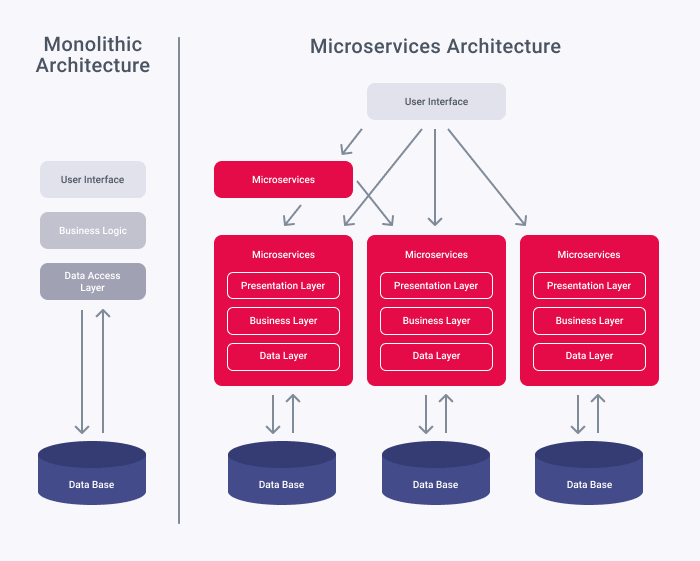
\includegraphics[width=0.85\textwidth]{img/microservice_architecture.png}
			\caption{Comparativa entre arquitectura de microservicios y arquitectura ``monolítica''. [\ref{bib_img: microservice architecture}]}
			\label{img: microservice architecture}
		\end{center}
	\end{figure}
	
	
	\pagebreak
	
	\section{Bases de datos}
	
	\noindent Para asegurar la persistencia de los datos en nuestra aplicación, es necesario utilizar una base de datos. En dicha base de datos, guardaremos información relevante para el correcto funcionamiento del sistema, en nuestro caso, redes y/o interfaces a monitorizar, o los datos monitorizados. \\
	
	\noindent En la aplicación de monitorización, distinguimos entre datos de dos tipos:
	
	\begin{itemize}
		\item Datos clásicos. Como por ejemplo, la información asociada a una red a monitorizar.
		\item Datos de tipo ''time series''. Como por ejemplo, las muestras de monitorización de una red.
	\end{itemize}

	\noindent En primer lugar, se diseña una base de datos tipo SQL para almacenar los ''datos clásicos''. Y por otro lado, se diseña una base de datos diferente, especializada para el almacenamiento de datos tipo ''time series'', en este caso, se elige una base de datos llamada InfluxDB.
	
	\subsection{Base de datos tipo relacional/SQL}
	
	\noindent SQL es una base de datos de tipo relacional. Dichas bases de datos, suponen una colección de información que organizan los datos en una serie de ''relaciones'' cuando la información es almacenada en una o varias ''tablas''. Por lo tanto, las relaciones suponen conexiones entre diferentes tablas, permitiendo así una asociación entre información diferente. [\ref{bib: relational database}] \\
	
	\noindent Por ejemplo, si vemos la figura \ref{img: example sql}, podemos comprobar como se realizan las relaciones entre las diferentes tablas (Ratings, Users, Movies o Tags), se realiza mediante uno de los campos definidos en la propia tabla. Por ejemplo, el campo ''user\_id'' de la tabla Ratings, permite una relación con la tabla Users, con el campo ''id''.
	
	\begin{figure}[h!]
		\begin{center}
			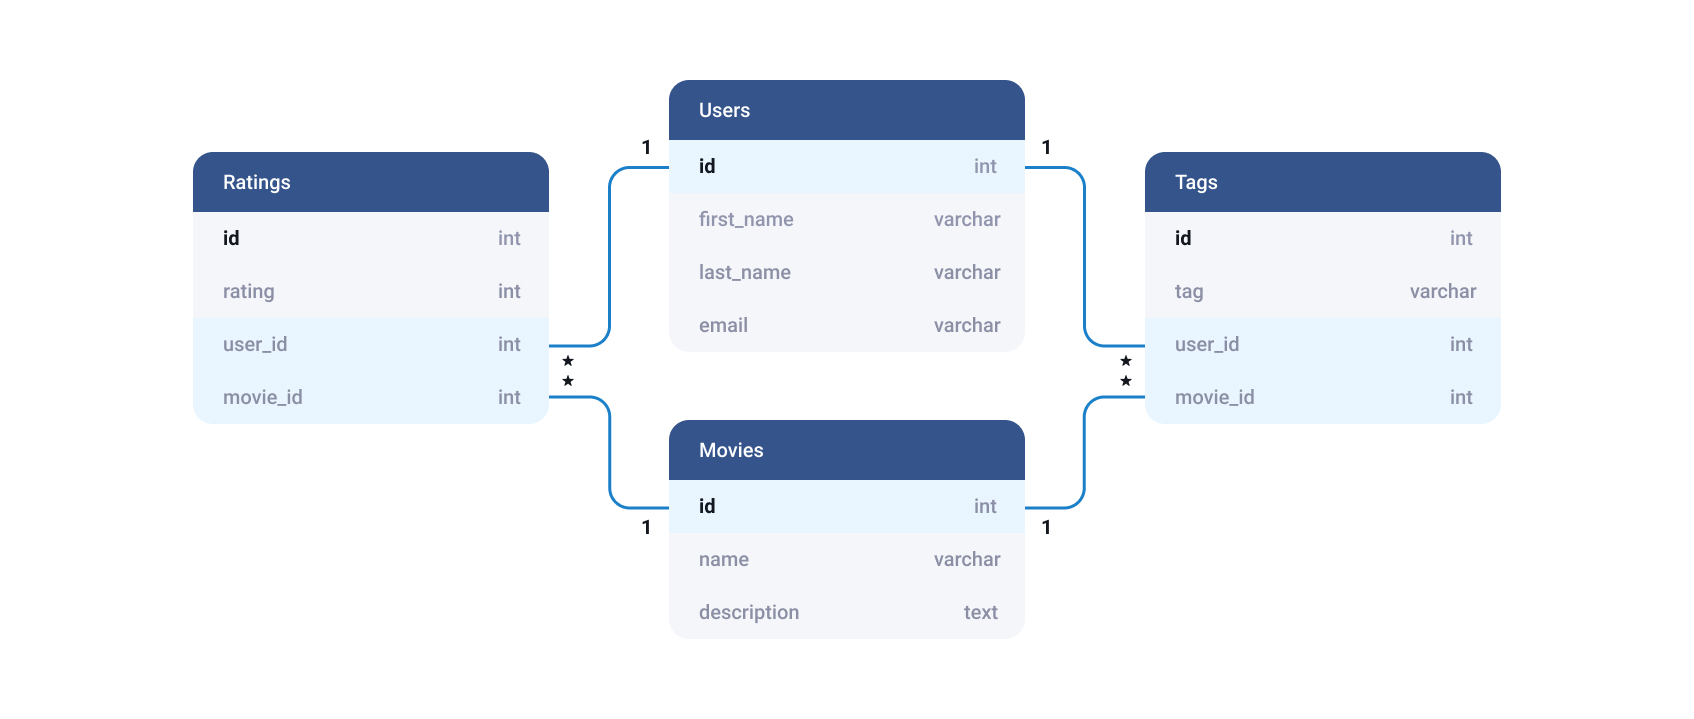
\includegraphics[width=0.95\textwidth]{img/example_relational_database.jpg}
			\caption{Ejemplo de relaciones dentro de una base de datos SQL. [\ref{bib_img: example sql}]}
			\label{img: example sql}
		\end{center}
	\end{figure}
	
	\noindent Para el caso de nuestra aplicación de monitorización de tráfico en red, modelamos la base de datos según la información que vamos a almacenar. Por lo que tenemos que definir la estructura de tablas, los campos que van a tener cada una de las tablas, y los campos por los que se van a relacionar entre sí. A esta información la llamamos modelo de datos.
	
	
	
	\pagebreak
	
	\subsection{Base de datos tipo ``time series''/InfluxDB} 
	
	\noindent InfluxDB es una base de datos diseñada para trabajar con datos tipo time-series. Si bien es cierto que SQL puede gestionar este tipo de datos, no fue creado estrictamente para este objetivo. En este caso, InfluxDB esta diseñado para almacenar grandes volúmenes de datos, y además realizar análisis en tiempo real sobre esos datos. \\
	
	\noindent En comparación con SQL, en InfluxDB un ``timestamp'' identifica un punto en cualquier serie de datos. Esto sería equivalente a SQL, si la clave primaria de una tabla es establecida por el sistema y siempre es equivalente al tiempo. Además, InfluxDB permite reconocer el ``schema'' de manera dinámica, además de que no estas obligado a definir el ``schema'' y seguirlo, es decir, se permiten cambios dentro de la misma serie de datos. [\ref{bib: influxdb doc vs sql}] \\
	
	\noindent Algunas de las razones destacadas para elegir InfluxDB son: [\ref{bib: influxdb doc}]
	
	\begin{itemize}
		\item Perfecto para almacenar datos de telemetría, como métricas de aplicaciones o sensores IoT.
		\item Los datos son comprimidos automáticamente para ser eficientes con el espacio disponible.
		\item Se realizan tareas automáticas de ``downsampling'' para reducir el uso de disco.
		\item Lenguaje para hacer consultas que permite analizar en profundidad los datos almacenados.
		\item Disponible una aplicación web para realizar consultas y comprobar los datos disponibles en la base de datos.
	\end{itemize}

	\vspace{10px}

	\noindent \textbf{\large Terminología} \\
	
	\noindent Comparando con los conceptos ya existentes en bases de datos de tipo SQL, se definen los siguientes conceptos en InfluxDB:
	
	\begin{itemize}
		\item ``measurement'': equivalente a una tabla.
		\item ``tags'': equivalente a columnas indexadas dentro de una tabla.
		\item ``fields'': equivalente a columnas no indexadas dentro de una tabla.
		\item ``points'': similar a las filas en una tabla.
	\end{itemize}

	\vspace{20px}

	\begin{figure}[h!]
		\begin{center}
			
\includegraphics[width=0.6\textwidth]{img/InfluxDB.png}
			\caption{Logotipo base de datos InfluxDB [\ref{bib_img: influxdb logo}].}
			\label{img: influxdb logo}
		\end{center}
	\end{figure}

	\pagebreak
	
	%\section{Modelo de predicción}
	% TODO: eliminar?
	
	\pagebreak
	
	\section[Lenguajes y frameworks]{Lenguajes de programación y frameworks}
	
	\noindent En resumen, para el desarrollo de esta aplicación se ha utilizado el lenguaje de programación Python, con el framework de desarrollo para APIs llamado FastAPI.
	
	\subsection{Python}
	
	\noindent Python [\ref{bib: python doc}] es un lenguaje de programación orientado a objetos, interpretado y de alto nivel con tipado dinámico. Es muy atractivo ya que permite un desarrollo rápido de aplicaciones, además de ser muy adecuado para realizar tareas de ``scripting''. Python es un lenguaje simple y sencillo de aprender. Por otro lado, dispone de multitud de ``librerías'' o ``módulos'' publicados por usuarios, dando lugar a una gran comunidad y una gran variedad de alternativas para implementar soluciones. \\
	
	\noindent Actualmente, Python destaca como lenguaje de programación en los siguientes ámbitos:
	\begin{itemize}
		\item Desarrollo de aplicaciones web, utilizando los frameworks Django, Flask o FastAPI.
		\item Tareas asociadas a ``data science'', utilizando librerías como Pandas o NumPy.
		\item Inteligencia artificial, utilizando frameworks como TensorFlow o scikit-learn.
	\end{itemize}
	
	\begin{figure}[h!]
		\begin{center}
			
\includegraphics[width=0.5\textwidth]{img/python_logo.png}
			\caption{Logotipo Python [\ref{bib_img: python logo}].}
			\label{img: python logo}
		\end{center}
	\end{figure}
	
	\subsection{FastAPI}
	
	\noindent FastAPI [\ref{bib: fastapi doc}] es un framework moderno y rápido para construir APIs utilizando la versión de Python 3.7+. Algunas de las características más destacadas son:
	
	\begin{itemize}
		\item Rápido: rendimiento muy alto, prácticamente a la par con otros lenguajes de programación destinados al desarrollo de backend (como NodeJS o Go).
		\item Intuitivo: soporta auto completado en el código.
		\item Robusto: código pensado para entornos de producción, además de incluir documentación automática (usando Swagger o ReDoc).
		\item Basado en estándares: al utilizar estándares de tipo de datos, permite ser totalmente compatible con los estándares de \href{https://github.com/OAI/OpenAPI-Specification}{OpenAPI} [\ref{bib: openapi}] y \href{https://json-schema.org/}{JSON Schema} [\ref{bib: json schema}].
	\end{itemize}
	
	\pagebreak
	
	\begin{figure}[h!]
		\begin{center}
			
\includegraphics[width=0.6\textwidth]{img/fastapi_logo.png}
			\caption{Logotipo FastAPI [\ref{bib_img: fastapi logo}].}
			\label{img: fastapi logo}
		\end{center}
	\end{figure}

	\subsection{Prophet}
	
	\noindent Prophet [\ref{bib: prophet doc}] es un framework del lenguaje de programación Python, desarrollado por \href{https://github.com/facebook/}{Meta}, que recoge una serie de procedimientos que permiten realizar predicciones de un dataset de series temporales, en el que se pueden encontrar diferentes efectos no lineales, llamados tendencias (como puede ser una tendencia anual, semanal, o mensual), además de otros efectos causados por fechas concretas. \\
	
	\noindent Es un framework de predicción basado en inferencia estadística, lo que permite tener un rendimiento mayor que si utilizamos técnicas de Machine Learning para solucionar el mismo problema de predicción de datos. Además, es robusto a datos no disponibles y a modificaciones aleatorias sobre las tendencias. 
	
	\begin{figure}[h!]
		\begin{center}
			
\includegraphics[width=0.55\textwidth]{img/prophet_logo.png}
			\caption{Logotipo Prophet [\ref{bib_img: prophet logo}].}
			\label{img: prophet logo}
		\end{center}
	\end{figure}
	
	\pagebreak
	
	\section[Despliegue en Producción]{Tecnologías utilizadas en un despliegue en producción}
	
	\noindent Otro de los aspectos importantes para la realización de este proyecto, es el hecho de que la aplicación desarrollada debe ser apta para desplegarse en un entorno de producción y funcionar correctamente para que sea implementada como microservicio por otras aplicaciones. Es por este motivo por el que nos decantamos por implementar este microservicio dentro de un contenedor. \\
	
	\noindent \textbf{\large Docker} \\

	\noindent Utilizamos Docker como la tecnología para realizar un contenedor de nuestra aplicación, implementando dentro del contenedor todas las librerías y código necesario para hacer funcionar la aplicación. \\
	
	\noindent Por otro lado, también será necesario desplegar diferentes contenedores que tendrán alojadas las bases de datos que utilizaremos en el proyecto. En este caso, al utilizar dos bases de datos, tendremos que hacer uso de un contenedor para desplegar una base de datos SQL, y otro contenedor para desplegar una base de datos InfluxDB. \\ 
	
	\noindent Los contenedores Docker necesarios se desplegarán sobre una máquina host que tenga en funcionamiento el ``daemon'' de Docker. 
	
	% TODO: revisar imagen
	\begin{figure}[h!]
		\begin{center}
			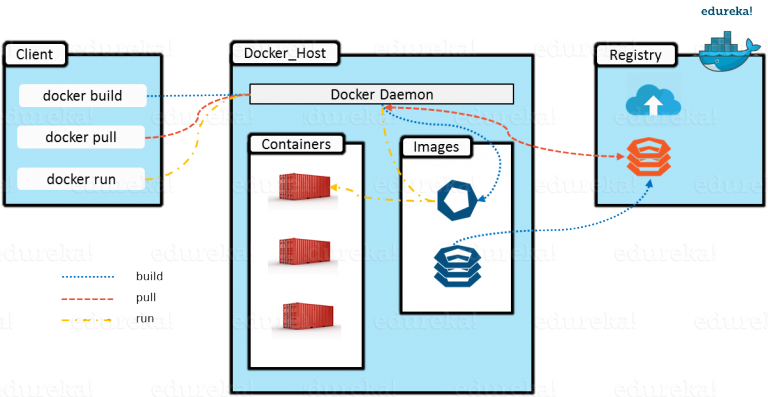
\includegraphics[width=1\textwidth]{img/docker_capture.png}
			\caption{Docker}
			%\label{img: prophet logo}
		\end{center}
	\end{figure}

	\pagebreak
	
	\noindent \textbf{\large Docker Compose} \\
	
	\noindent Compose es una herramienta de Docker que permite definir y ejecutar instancias multi contenedores de Docker [\ref{bib: docker compose doc}]. Con la herramienta Compose, podemos utilizar un archivo YAML para describir y configurar los contenedores que vamos a utilizar, dando lugar a que con un único comando puedas crear y ejecutar todos los servicios de la aplicación, y con la misma configuración. \\
	
	\noindent Compose funciona para los diferentes entornos: producción, desarrollo, y o pruebas. Además, tiene disponibles comandos para hacer más sencilla la tarea de iniciar o parar servicios, o ver la salida de consola producida por los contenedores. \\
	
	\noindent En el caso de nuestra aplicación, el archivo ``\textit{docker-compose.yml}'' utilizado para el entorno de desarrollo sería el siguiente:
	
	\begin{lstlisting}[style=yaml, caption={Archivo configuración de contenedores para entorno de desarrollo.}]
version: '3.8'

services:
  traffic_forecast:
    build: ./backend
    ports:
     - 5000:5000
    environment:
     - POSTGRES_USER=monitor
     - POSTGRES_PASSWORD=forecast2022
     - POSTGRES_DB=traffic-forecast
     - INFLUX_TOKEN=*******
     - INFLUX_ORG=e-lighthouse
     - INFLUX_BUCKET=traffic-forecast
     - SECRET_KEY=upct2022_sk
     - FASTAPI_CONFIG=development
    volumes:
     - ./backend:/app
    depends_on:
     - db
     - influxdb

  db:
    image: postgres:13
    expose:
     - 5432
    environment:
     - POSTGRES_USER=monitor
     - POSTGRES_PASSWORD=forecast2022
     - POSTGRES_DB=traffic-forecast
    volumes:
     - ./data/postgres_db:/var/lib/postgressql/data
    
   influxdb:
     image: influxdb:latest
     volumes:
       - ./data/influxdb/data:/var/lib/influxdb2:rw
     ports:
       - 8086:8086
	\end{lstlisting}

	\pagebreak
	
	\noindent Para desplegar los contenedores, según el archivo YAML definido, tenemos que ejecutar el siguiente comando: 
	
	\begin{verbatim}
		docker compose up -f <filename> traffic_forecast
	\end{verbatim}
	
	\noindent \textbf{\large Traefik} \\
	
	\noindent Traefik es una herramienta que permite hacer de ``reverse proxy'' y ``load balancer'' en contenedores Docker, permitiendo el despliegue sencillo de microservicios en un entorno de producción. \\
	
	\noindent Traefik esta diseñado para ser simple de operar, pero con una gran capacidad de gestión en entornos complejos. Además, se integra perfectamente con la infraestructura ya existente y configurar el sistema de manera dinámica. Algunas de las tareas que realiza Traefik son: [\ref{bib: traefik webpage}] 
	
	\begin{itemize}
		\item Gestionar middlewares necesarios para la aplicación (forzar protocolos específicos, configurar contraseña para el servicio...).
		\item Funcionar con API Gateway, gestionando los dominios y certificados para cada uno de los microservicios desplegados.
		\item Orquestador de nodo de entrada, gestionando la comunicación de tráfico de un dominio hacia el servicio asociado.
	\end{itemize}

	% TODO: revisar imagen
	\begin{figure}[h!]
		\begin{center}
			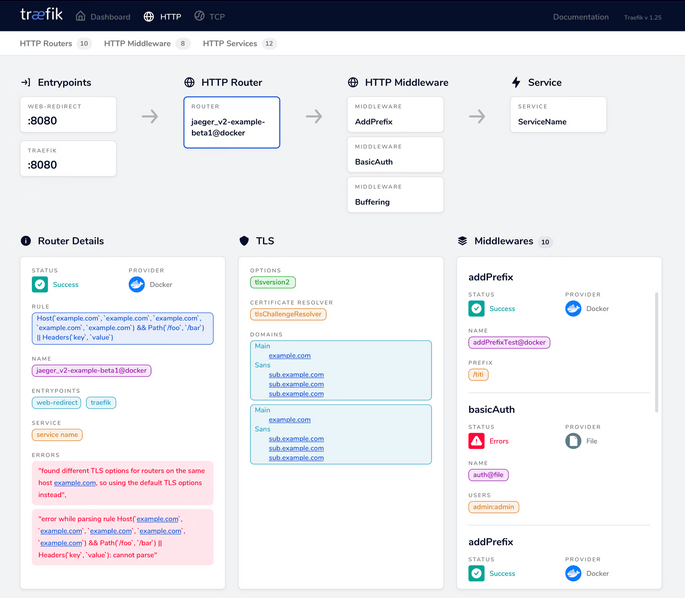
\includegraphics[width=0.78\textwidth]{img/traefik_example.png}
			\caption{Captura portal de gestión de Traefik. Detalle de enrutado hacia un servicio.}
			%\label{img: prophet logo}
		\end{center}
	\end{figure}
	
	\pagebreak
	
	\noindent En el caso de nuestra aplicación, para el entorno de producción usamos el siguiente archivo que permite a la herramienta docker compose ejecutar los servicios con sus configuraciones asociadas. Como podemos ver, en la sección de ``labels'' se encuentra la configuración asociada a Traefik. Dicha configuración permite a Traefik asignar un servicio a un dominio, crear un certificado SSL y configurar los puertos de acceso para dicho servicio. [\ref{bib: traefik wiki}]
	
	\begin{lstlisting}[style=yaml, caption={Archivo configuración de contenedores para entorno de producción.}]
version: '3.8'

services:
  traffic_forecast:
    build: ./backend
    container_name: traffic_forecast-api
    restart: unless-stopped
    environment:
      - POSTGRES_USER=monitor
      - POSTGRES_PASSWORD=forecast2022
      - POSTGRES_DB=traffic-forecast
      - INFLUX_URL=https://tfm-influx.ranii.pro:8443/
      - INFLUX_TOKEN=****
      - INFLUX_ORG=e-lighthouse
      - INFLUX_BUCKET=traffic-forecast
      - SECRET_KEY=upct2022_sk
    volumes:
      - ./backend:/app
    labels:
      - traefik.enable=true
      - traefik.http.routers.tf-api.entryPoints=web-secure
      - traefik.http.routers.tf-api.rule=Host(`tfm-api.ranii.pro`)
      - traefik.http.routers.tf-api.tls.certresolver=default
      - traefik.http.services.tf-api.loadbalancer.server.port=5000
    depends_on:
      - db
      - influxdb

  db:
    image: postgres:13
    container_name: traffic_forecast-postgres
    restart: unless-stopped
    environment:
      - POSTGRES_USER=monitor
      - POSTGRES_PASSWORD=forecast2022
      - POSTGRES_DB=traffic-forecast
    volumes:
      - ./data/postgres_db:/var/lib/postgressql/data

  influxdb:
    image: influxdb:latest
    container_name: traffic_forecast-influx
    restart: unless-stopped
    volumes:
      - ./data/influxdb/data:/var/lib/influxdb2:rw
    labels:
      - traefik.enable=true
      - traefik.http.routers.tf-influx.entryPoints=web-secure
      - traefik.http.routers.tf-influx.rule=Host(`tfm-influx.ranii.pro`)
      - traefik.http.routers.tf-influx.tls.certresolver=default
      - traefik.http.services.tf-influx.loadbalancer.server.port=8086
	\end{lstlisting} 

	\noindent Para desplegar los contenedores, según el archivo YAML definido, tenemos que ejecutar el siguiente comando: 
	
	\begin{verbatim}
		docker compose up -f <filename> traffic_forecast
	\end{verbatim}

	\noindent En el caso de querer profundizar más en el funcionamiento de Traefik, se puede consultar el siguiente enlace \href{https://doc.traefik.io/traefik/}{Traefik: Get Started}
	
	\chapter{Diseño e implementación del sistema}
	
	\section{Descripción REST API}
	
	\section{Estructura de la aplicación}
	
	\section{Modelos de datos}
	
	\subsection{Base de datos SQL}
	
	\subsubsection{Modelos de datos}
	
	\noindent El primer modelo de datos de la aplicación, es el referido a la información de una red a monitorizar. La descripción del modelo la podemos ver en la figura \ref{img: modelo sql networks}.
	
	\begin{figure}[h!]
		\begin{center}
			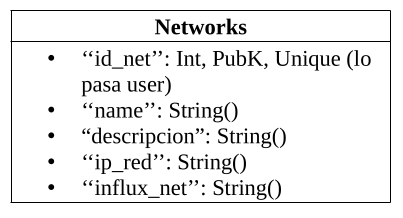
\includegraphics[width=0.5\textwidth]{img/model_sql_networks.png}
			\caption{Modelo de datos para las redes a monitorizar. Equivale con la tabla ''networks''.}
			\label{img: modelo sql networks}
		\end{center}
	\end{figure}
	
	\noindent El segundo modelo de datos de la aplicación, es el referido a la información de una interfaz a monitorizar, que esta dentro de una red monitorizada. La descripción del modelo la podemos ver en la figura \ref{img: modelo sql interfaces}.
	
	\begin{figure}[h!]
		\begin{center}
			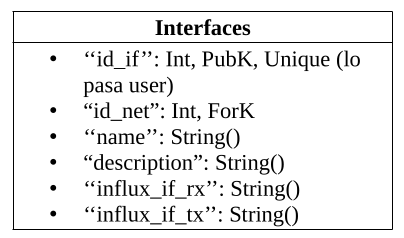
\includegraphics[width=0.5\textwidth]{img/model_sql_interfaces.png}
			\caption{Modelos de datos para las interfaces a monitorizar. Equivale con la tabla ''interfaces''}
			\label{img: modelo sql interfaces}
		\end{center}
	\end{figure}
	
	\noindent Se establece una relación del modo que una interfaz solo puede pertenecer a una red monitorizada, y que además, una red monitorizada puede tener muchas interfaces. Dicha relación se realiza mediante el campo ''id\_net'' de la tabla Interfaces. \\
	
	\noindent Por último, la base de datos SQL utilizada para esta aplicación es PostgreSQL [\ref{bib: postgresql}], ya que además de ser Open Source, permite una gran escalabilidad, amoldándose a los recursos de la máquina en la que esté funcionando.
	
	\subsection{Base de datos InfluxDB}
	
	\noindent \textbf{\large Modelo de datos} \\
	
	\noindent Para la aplicación a diseñar, se plantea la premisa de que en la base de datos InfluxDB solo se van a guardar los datos de cada muestra de monitorización de una interfaz. Además, se pueden tener tantas redes como sean necesarias, y dentro de cada red, tantas interfaces como creamos necesarias. \\
	
	\noindent En resumen, definimos el modelo de datos que tiene que seguir nuestra aplicación:
	
	\begin{itemize}
		\item ``measurement'': equivalente a una red a monitorizar, valor almacenado en Networks::influx\_net.
		\item ``fields'': nombre del valor a monitorizado, en este caso el default es \textit{link\_count}.
		\item ``tags'': solo tenemos un tag llamado \textit{interface}, su objetivo es identificar a que interfaz pertenece el punto de monitorización. El valor puede estar ser Interfaces::influx\_if\_rx o Interfaces::influx\_if\_tx.
		\item ``points'': corresponde con el valor numérico del ``field''. En este caso, corresponde con el valor númerico de link\_count en ese periodo de 5 minutos.
	\end{itemize} 
	
	\section{Endpoints}
	
	\section{Implementación del sistema}
	
	\pagebreak
	
	\chapter{Pruebas y validación del sistema}
	
	\pagebreak
	
	\chapter{Conclusiones}
	
	\section{Propuestas futuras}
	
	\pagebreak
	
	\chapter{Bibliografía}
	
	\subsection*{Enlaces y referencias}
	\addcontentsline{toc}{section}{Enlaces y referencias}
	
	\begin{enumerate}
		% 1
		\item
		\label{bib: what is api}
		\href{https://aws.amazon.com/es/what-is/api/}{¿Qué es una API?}
		
		% 2
		\item
		\label{bib: microservices}
		\href{https://learn.microsoft.com/en-us/azure/architecture/guide/architecture-styles/microservices}{Microservice architecture style}
		
		
		% 3
		\item
		\label{bib: relational database}
		\href{https://cloud.google.com/learn/what-is-a-relational-database}{What is a relational database?}
		
		
		% 4
		\item
		\label{bib: postgresql}
		\href{https://www.postgresql.org/}{PostgreSQL}
		
		% 5
		\item
		\label{bib: influxdb doc}
		\href{https://www.stackhero.io/en/services/InfluxDB/documentations/Introduction#differences-between-influxdb-and-relational-sql-databases}{InfluxDB: Introduction}
		
		% 6
		\item
		\label{bib: influxdb doc vs sql}
		\href{https://archive.docs.influxdata.com/influxdb/v1.2/concepts/crosswalk/}{InfluxDB: Comparison to SQL}
		
		% 7
		\item
		\label{bib: python doc}
		\href{https://www.python.org/}{Python}
		
		% 8
		\item
		\label{bib: fastapi doc}
		\href{https://fastapi.tiangolo.com/}{FastAPI framework}
		
		% 9
		\item
		\label{bib: openapi}
		\href{https://github.com/OAI/OpenAPI-Specification}{GitHub: OpenAPI-Specification}
		
		% 10
		\item
		\label{bib: json schema}
		\href{https://json-schema.org/}{JSON Schema}
		
		% 11
		\item
		\label{bib: prophet doc}
		\href{https://facebook.github.io/prophet/}{Prophet}
		
		% 12
		\item
		\label{bib: docker compose doc}
		\href{https://docs.docker.com/compose/}{Docker Compose Overview}
		
		% 13
		\item
		\label{bib: traefik webpage}
		\href{https://traefik.io/traefik/}{Traefik Webpage}
		
		% 14
		\item
		\label{bib: traefik wiki}
		\href{https://doc.traefik.io/traefik/}{Traefik Wiki}
		
		
	\end{enumerate}

	\vspace{20px}
	
	\subsection*{Figuras}
	\addcontentsline{toc}{section}{Imagenes}

	\begin{enumerate}
		
		% 1
		\item
		\label{bib_img: microservice architecture}
		\href{https://xbsoftware.com/blog/microservices-vs-monolithic-architecture/}{Monolithic vs Microservices Architecture}
		
		% 2
		\item
		\label{bib_img: example sql}
		\href{https://xbsoftware.com/blog/main-types-of-database-management-systems/}{Relational Databases}
		
		% 3
		\item
		\label{bib_img: influxdb logo}
		\href{https://www.influxdata.com/}{InfluxDB}
		
		% 4
		\item
		\label{bib_img: python logo}
		\href{https://www.python.org/}{Python}
		
		% 5
		\item
		\label{bib_img: fastapi logo}
		\href{https://fastapi.tiangolo.com/}{FastAPI}
		
		% 6
		\item
		\label{bib_img: prophet logo}
		\href{https://facebook.github.io/prophet/}{Prophet}
		
		
	\end{enumerate}
	
	\pagebreak
	
	\chapter*{Anexos}
	\addcontentsline{toc}{chapter}{Anexos}
	
	\section*{Anexo I. Generación dataset sintético}
	\addcontentsline{toc}{section}{Anexo I. Generación dataset sintético}
	
\end{document}